\documentclass[10pt]{article}
\usepackage{wrapfig}
%\usepackage{epsf}
\usepackage{fancyhdr,epsfig,graphics,tabularx,times}
\usepackage{amsmath}
\usepackage{amssymb}
\usepackage{palatino}
%\usepackage[dvips]{graphics}
\usepackage{fancyhdr}
\usepackage{epsfig}
\usepackage{multirow}
\usepackage{cancel}
\usepackage[bookmarks]{hyperref}
\usepackage{longtable}
\usepackage{soul}
\parindent 0in
\parskip 1ex
\oddsidemargin  0in
\evensidemargin 0in
\textheight 8.5in
\textwidth 6.5in
\topmargin -0.25in
\setcounter{section}{0}

\pagestyle{fancy}
\lhead{\bf BME354L: Introduction to Medical Instrumentation}
\rhead{\bf Nightingale (Spring 2015)}
\cfoot{\thepage}



\begin{document}
\section*{Problem Set \#3: Detection Circuits and Filters}

\textbf{DUE:} Monday, 2013-02-10 at 5:00 PM in the grader box

\begin{enumerate}
\item {\bf Tuned RLC dividers}, as shown below, can be used to determine changes in capacitive
transducers.  
\begin{enumerate}
\item Generate plots of the magnitude and phase of the transfer function
($\bar{V}_{out}/\bar{V}_{in}$) for $\omega =$ 1000 krad/s, $R$ = 100 $\Omega$
and $L$ = 1 mH for 0.5 $< C <$ 1.5 nF.  Be sure to include your work to derive
the transfer function, along with any code used to generate your plots (don't
forget to label your axes with units!).  \footnote{Self-check hint: make sure
your plots agree with your analytic solution for the resonant frequency of this
circuit.} 

\item Explain how the phase response of this divider is used to measure capacitive transducer changes. 

\item What role does the resistor play in ``tuning'' this divider? 

\item What is the maximum sensitivity of this circuit?

\end{enumerate}

\begin{center}
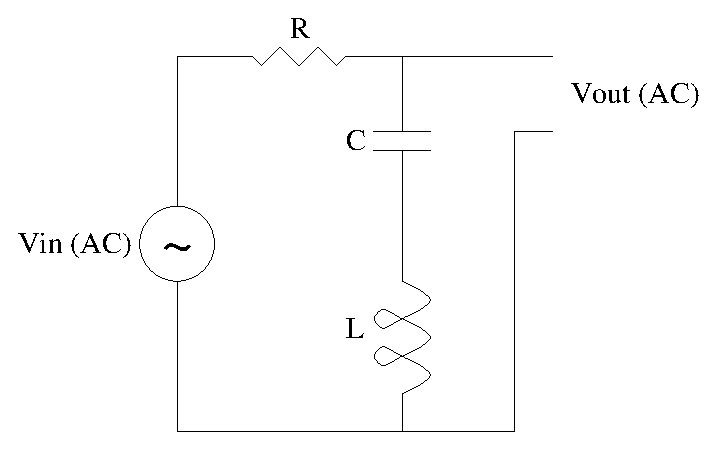
\includegraphics[scale=0.75]{tunedrlc.eps}
\end{center}

\item Consider the {\bf reactance bridge circuit} below; derive an expression for
$C_2$ in terms of $C_1$, $R_1$ and $R_2$ to balance this bridge (i.e.,
$V_\textrm{out} = 0$).

\begin{center}
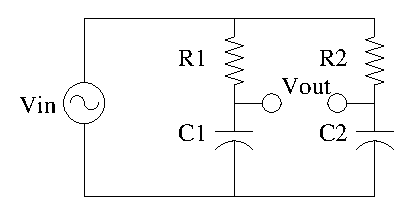
\includegraphics{reactance_bridge.eps}
\end{center}

\item {\bf First-Order Filter Design} Ultrasound scanners operate on
signals that range from 1 - 10 MHz, but typically face significant noise $\leq$
100 Hz.

\begin{enumerate}
\item Design a passive first-order filter using a capacitive element that:
\begin{itemize}
    \item Attenuates noise $\leq$ 100 Hz at least -40 dB relative to the desired passband of 1 - 10 MHz, and
    \item does not distort the passband more than 15$^\circ$.
\end{itemize}

Make sure that you:
\begin{itemize}
    \item Draw the circuit diagram with specified component values.
    \item Explicitly state the magnitude and phase expressions for the transfer function.
    \item Draw the magnitude and phase Bode plots, and indicate the passband region and the region of noise being attenuated.
    \item What is the input impedance of your filter?
\end{itemize}
\item Repeat the same design process as above for a passive first-order filter using an inductive element.  Present the same circuit diagram, transfer functions, labeled Bode plots, and input impedance analysis. 
\item Comment on any differences between the behavior of the two passive
filters.  Most of the filters that we construct in lab use capacitive, instead
of inductive, elements; why might this be?\footnote{ This will
require a literature search (which these days means an Internet search).  Please cite all sources!}
\end{enumerate}

\item {\bf Bandpass Filter Design} Electromyography (EMG) signals
tend to have biopotential voltages ranging from 10$^{-5}$ - 10$^{-1}$ V over a
frequency range of 50 - 5000 Hz.  Assuming that you have a single op amp with a
maximum output voltage of +10V, design a bandpass filter that will amplify the
EMG to the maximum possible gain without exceeding the op amp's linear range of
operation.  Sketch the amplitude and phase Bode plots for this filter.

\end{enumerate}

\end{document}
